\documentclass[conf]{new-aiaa}
%\documentclass[journal]{new-aiaa} for journal papers
\usepackage[utf8]{inputenc}

\usepackage{graphicx}
\usepackage{amsmath}
\usepackage[version=4]{mhchem}
\usepackage{siunitx}
\usepackage{longtable,tabularx}
\setlength\LTleft{0pt}

\title{Multidisciplinary Optimization of a Turboelectric Tiltwing Urban Air Mobility Aircraft}

\author{Eric S. Hendricks\footnote{Aerospace Engineer, Propulsion Systems Analysis Branch, 21000 Brookpark Rd MS 5-11.}, Robert D. Falck\footnote{Aerospace Engineer, Mission Analysis and Architecture Branch, 21000 Brookpark Rd MS 162-2, AIAA Member.}, Justin S. Gray \footnote{Aerospace Engineer, Propulsion Systems Analysis Branch, 21000 Brookpark Rd MS 5-11, AIAA Member}, Eliot D. Aretskin-Hariton\footnote{Aerospace Engineer, Intelligent Control and Autonomy Branch, 21000 Brookpark Rd MS 77-1.}, Daniel J. Ingraham \footnote{Aerospace Engineer, Acoustics Branch, 21000 Brookpark Rd MS 54-3}, \\ Jeffryes W. Chapman\footnote{Aerospace Engineer, Propulsion Systems Analysis Branch, 21000 Brookpark Rd MS 5-11.}, Sydney L. Schnulo\footnote{Aerospace Engineer, Propulsion Systems Analysis Branch, 21000 Brookpark Rd MS 5-11.}, Jeffrey C. Chin\footnote{Aerospace Engineer, Propulsion Systems Analysis Branch, 21000 Brookpark Rd MS 5-11.}, John P. Jasa\footnote{Aerospace Engineer Intern, Propulsion Systems Analysis Branch, 21000 Brookpark Rd MS 5-11 and Ph.D. Candidate, University of Michigan.}, and Jennifer D. Bergeson\footnote{Aerospace Engineer Intern, Propulsion Systems Analysis Branch, 21000 Brookpark Rd MS 5-11 and Undergraduate Student, Purdue University.}}
\affil{NASA Glenn Research Center, Cleveland, OH, 44135}

\begin{document}

\maketitle



% Main point: Developing a new multidisciplinary approach/toolset for designing UAM vehicles which are highly coupled

% Baseline design process from Chris Silva and compare to our design process

% Focus on integration of disciplines and use of gradient-based optimization

% Demonstration problem summary and optimization formulation

% Demonstration problem results


% disciplines:
%   aerodynamics
%   structures/mass
%   propulsion (cycle/electrical/propeller)
%   trajectory
%



\begin{abstract}
Urban air taxis, also known as urban air mobility (UAM) vehicles, are anticipated to be an area of significant market growth in the near future.
These vehicles are typically vertical take-off and landing (VTOL) designs which are capable of carrying 1 to 30 passengers in an intra-urban environment with flights of less than 50 nautical miles.
Development of UAM vehicles and their integration into the airspace will be enabled by advancements in a number of areas including electrified propulsion systems, structures, acoustics, automation, and controls.
However, creating optimized designs for these unique vehicles with emerging technologies across these disciplines presents a new challenge.
This work describes the development of a multidisciplinary analysis environment which can be used to support the conceptual design of these UAM vehicles.
The tools included in this multidisciplinary analysis model the aircraft trajectory, vehicle aerodynamics, structures,  and electrified propulsion system.
The multidisciplinary analysis environment is then demonstrated in the design optimization of a turboelectric tiltwing UAM vehicle concept.
\end{abstract}

% \section{Nomenclature}

% {\renewcommand\arraystretch{1.0}
% \noindent\begin{longtable*}{@{}l @{\quad=\quad} l@{}}
% $A$  & amplitude of oscillation \\
% $a$ &    cylinder diameter \\
% $C_p$& pressure coefficient \\
% $Cx$ & force coefficient in the \textit{x} direction \\
% $Cy$ & force coefficient in the \textit{y} direction \\
% c   & chord \\
% d$t$ & time step \\
% $Fx$ & $X$ component of the resultant pressure force acting on the vehicle \\
% $Fy$ & $Y$ component of the resultant pressure force acting on the vehicle \\
% $f, g$   & generic functions \\
% $h$  & height \\
% $i$  & time index during navigation \\
% $j$  & waypoint index \\
% $K$  & trailing-edge (TE) nondimensional angular deflection rate
% \end{longtable*}}

\section{Introduction}\label{sec:intro}
% Text for the introduction section
\lettrine{F}{or} more than half a century, humans have envisioned a future where every person would have a personal air vehicle for transportation, often envisioned as a flying car.
Henry Ford stated in 1940: ``Mark my word: a combination airplane and motorcar is coming. You may smile, but it will come.''\cite{schilling2001looking}
While this future has yet to come to pass, recent developments in aviation and technology have made this reality closer than ever. 
The vision now is for an urban air taxi service (also commonly referred to as urban air mobility or UAM) capable of shuttling passengers around metropolitan areas thereby escaping the road congestion below.\cite{moore2003personal}
This vision has sparked the development of a number of UAM concept vehicles within industry and at NASA.
These vehicles are typically vertical take-off and landing (VTOL) designs which which are capable of carrying 1 to 30 passengers in an intra-urban environment on flights of less than 50 nautical miles. 

Within NASA, three UAM concept vehicles were initially developed by the Revolutionary Vertical Lift Program to focus and guide research activities.\cite{johnson2018concept}
These vehicles, shown in Figure \ref{f:UAM}, differ significantly in their design, size, payload, range, propulsion system and operation.
The concept on the left is a quadrotor vehicle designed to carry a single passenger over a short 50 nm range.  
Because of this short range and small size, it is anticipated that the propulsion system for this vehicle would be all-electric.
The vehicle on the right is the next largest with the ability to carry six passengers over four 50 nm flight segments before needing refueling.
% The mission profile for this vehicle (and the segments for the other vehicles) is shown in Figure \ref{f:profile}. 
This concepts is envisioned to have a hybrid propulsion system with some power produced by energy stored in batteries with the rest coming from turboshaft engines.
Lastly, the largest concept in the center is a tiltwing design capable of carrying 15 passengers on eight 50 nm flight segments.
The propulsion system for this concept is expected to be a turboelectric design where a single turboshaft engine generates electricity which is transmitted four electric motor driven rotors/propellers.
% The propulsion system for this turboelectric tiltwing concept is shown in Figure \ref{f:turboelectric}.
It is this last concept, the turboelectric tiltwing, which will serve as the demonstration example in this paper.

\begin{figure}
\begin{center}
 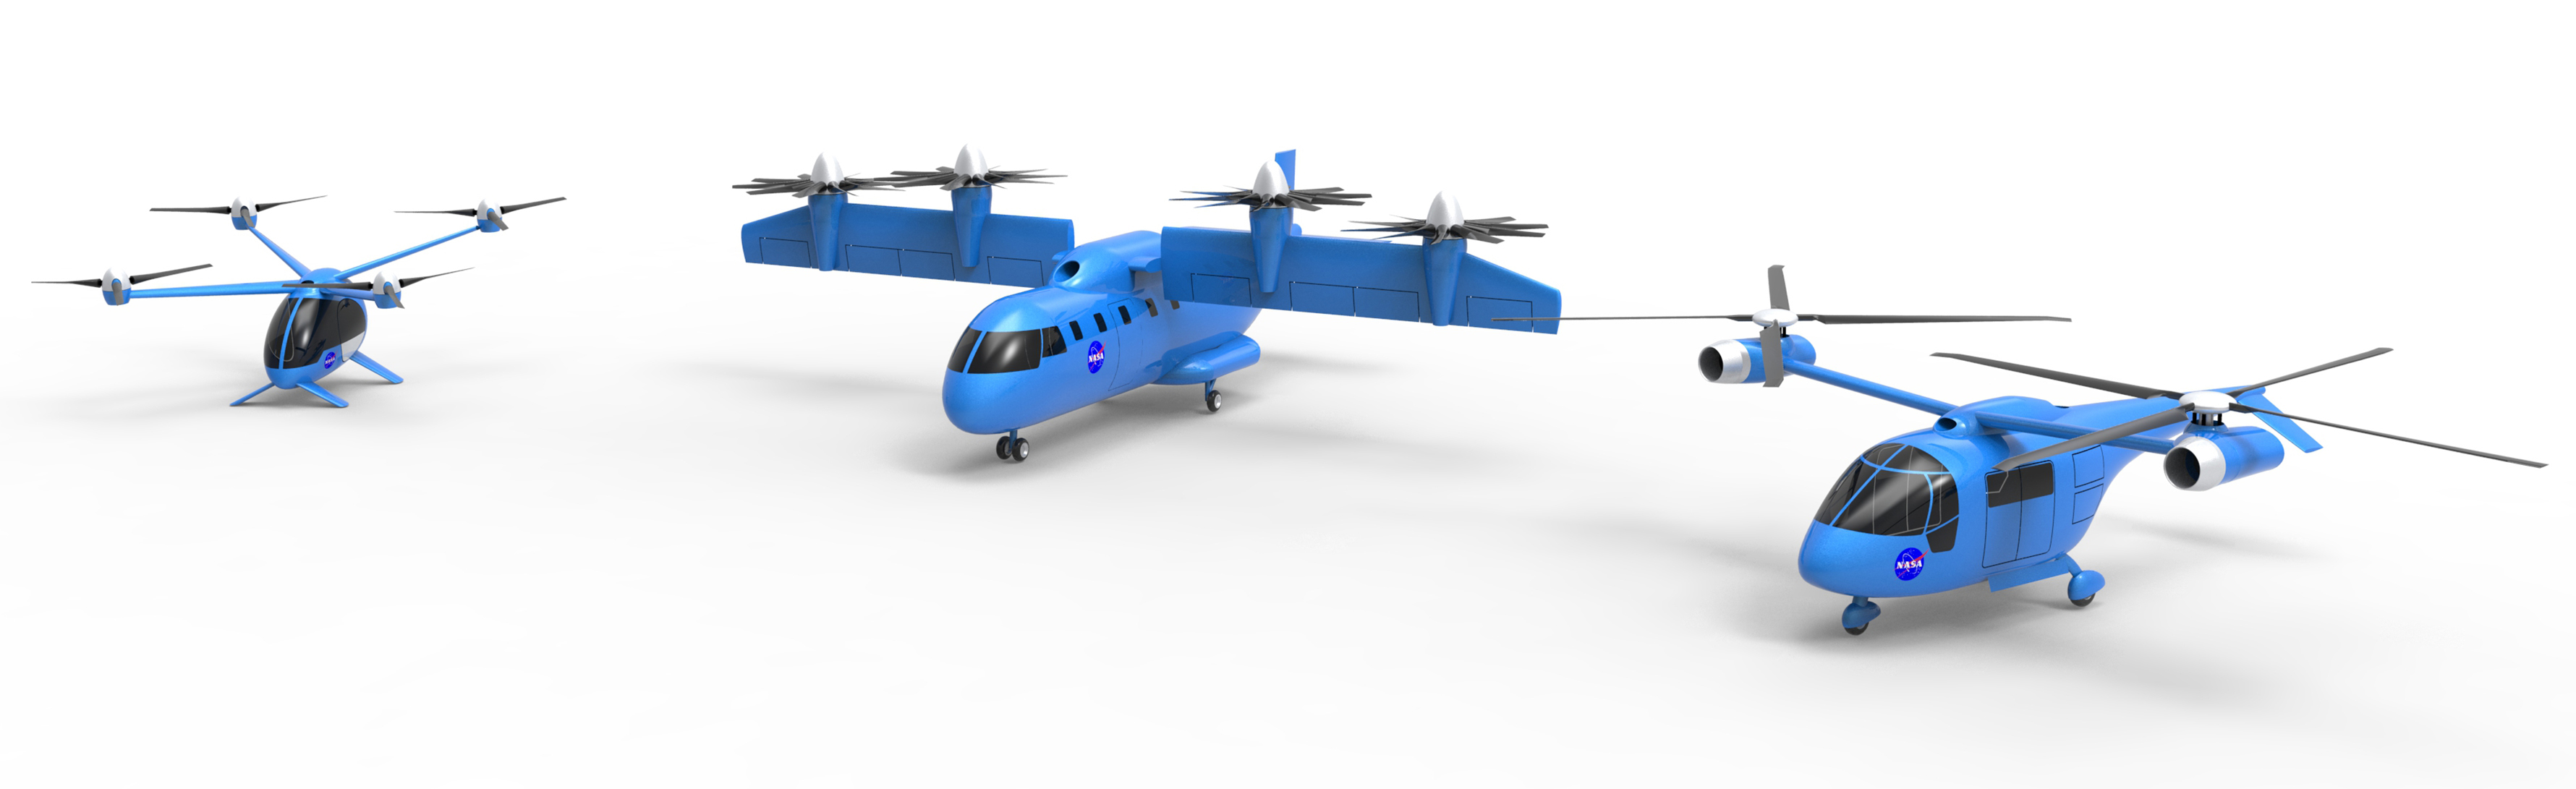
\includegraphics[width=1.0\textwidth]{../Images/UAM_GROUP1.jpg}
 \caption{NASA Urban Air Mobility Concept Vehicles.}
 \label{f:UAM}
\end{center}
\end{figure}

% \begin{figure}
% \begin{center}
%  \includegraphics[width=0.6\textwidth]{../Images/Mission_profile.pdf}
%  \caption{Mission Profiles for UAM Concept Vehicles.\cite{johnson2018concept}}
%  \label{f:profile}
% \end{center}
% \end{figure}


% The purpose behind NASA developing these designs is to focus and guide NASA research on the technologies needed to make UAM become a reality.\cite{johnson2018concept}
The initial studies to develop these UAM concept vehicle designs applied a set of existing rotorcraft design and analysis tools in a traditional design process.
Overall, the the objectives of these studies were to sufficiently refine the design such that crucial technologies and research needs could be identified. 
Asa result, the concept designs generated several areas of further research which are required to evolve and mature the designs were identified.
These areas included improving the modeling and assumptions for the propulsion system, vehicle weights, aerodynamics and acoustics.\cite{johnson2018concept}
Furthermore, it was identified that the traditional design process needs to be modified to perform an integrated multidisciplinary environment to optimize these concepts to further improve the overall design

Given these needs, this work presents the development of a multidisciplinary analysis environment which can be used to support the conceptual design of UAM vehicles.
This multidisciplinary analysis and design environment provides improved modeling capabilities for disciplines including modeling the aircraft trajectory, propulsion system, electrical system, structures and aerodynamics. %potentially add TMS and the acoustics if they end up in the models for this paper
These disciplinary modeling tools are developed with the ability to compute analytic derivatives to support the close coupling of the tools within a larger multidisciplinary environment.
The analytic computation of derivatives is a key feature of this tool suite as it provides enhanced capabilities for gradient-based optimization of the multidisciplinary model. 

This paper is organized as follows:
Section \ref{sec:trad_process} first presents the traditional design process and tools used in the initial design of the UAM concept vehicles.
Following this background, the development of the new multidisciplinary design, analysis and optimization (MDAO) environment and its supporting tools is summarized in Section \ref{sec:mdao_process}.
The features of the multidisciplinary analysis environment are then demonstrated by applying it to the optimization of the turboelectric tiltwing UAM vehicle described above in Section \ref{sec:opt_prob}.
Following this optimization demonstration, conclusions and future work are discussed in Section \ref{sec:conc}. 

 %Eric

\section{Traditional Design and Analysis Environment}\label{sec:trad_process}
% This file should contain text on the baseline design process and tools used by RVLT/Chris Silva for comparison to our new MDAO design process
% This section is assigned to Justin

Add a description of the traditional process and tools used by Chris Silva and team for developing the 3 UAM vehicle designs.  Include an XDSM of the traditional process.  

General outline for this section:
\begin{itemize}
    \item Traditional process used by RVLT for initial concept development applied different disciplinary tools in a linear/sequential fashion
    \item NPSS used to create cycle model and engine surrogate model
    \item CAMRAD used to model the rotors
    \item ...tools for other disciplines...
    \item NDARC used to determine mission performance
    \item Optimization/iterations completed using this tool set to generate initial designs
    \item Challenges:
    \begin{itemize}
        \item Process does not include detailed models for some disciplines (electrical?)
        \item Existing tool set does not provide capabilities for completing large scale gradient-based optimization to further refine the designs
    \end{itemize}
\end{itemize}


\begin{figure}[htb]
\begin{center}
 \textbf{!!!!! Create XDSM of Traditional Process !!!!!}
 % 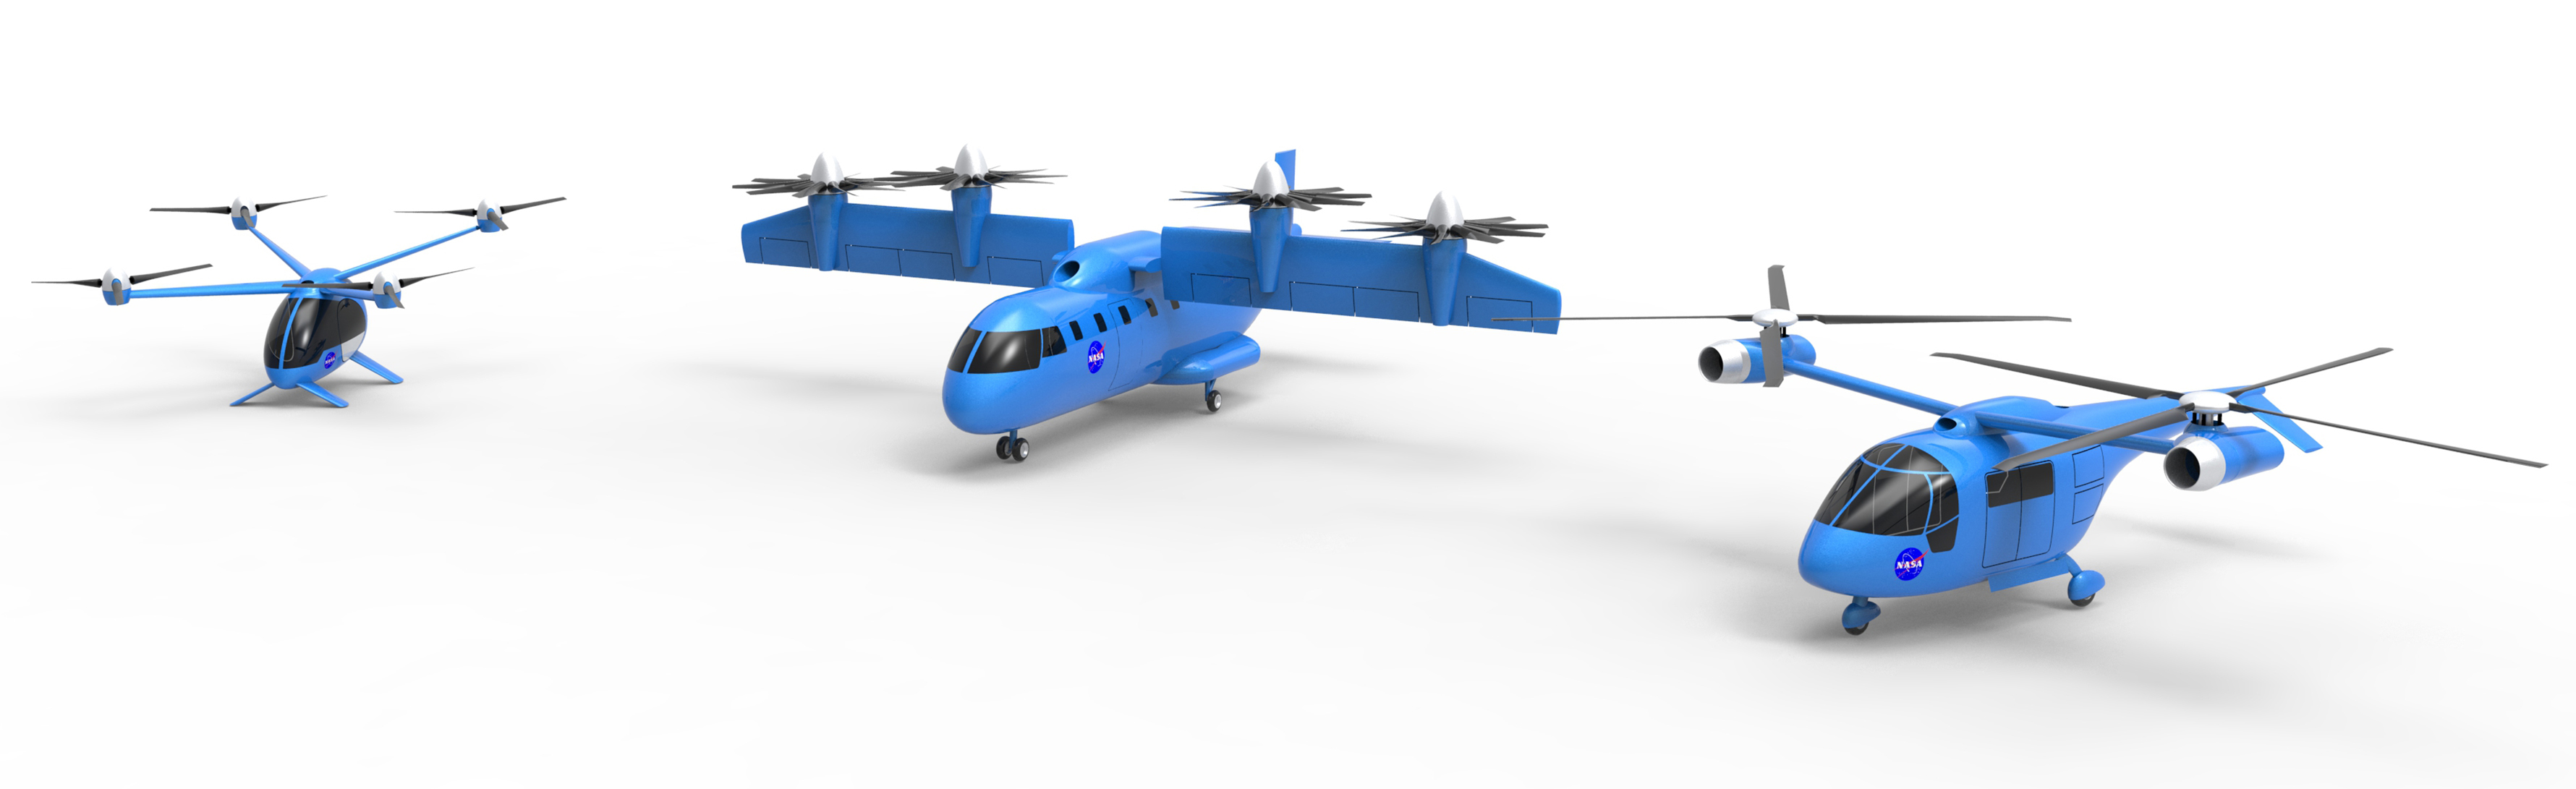
\includegraphics[width=1.0\textwidth]{../Images/UAM_GROUP1.jpg}
 \caption{Traditional Conceptual Design Process.}
 \label{f:trad_XDSM}
\end{center}
\end{figure}

 %Justin

\section{Multidisciplinary Design, Analysis, and Optimization Environment}\label{sec:mdao_process}
% The text in this file should contain an overview of the new MDAO environment/process we are developing as well as OpenMDAO

As stated in the Introduction, the UAM concept development to date has focused on identifying a set of vehicle designs and the discipline areas where further refinement is needed to improve the designs.
Given the multidisciplinary design challenges presented by these new UAM vehicle concepts, the objective of this research is to develop a multidisciplinary analysis and optimization environment capable of addressing these needs.
This analysis environment therefore needs to contain separate analysis tools for each of the disciplines under consideration.
Furthermore, these disciplinary tools needs to be tightly integrated to enable the optimization of the overall vehicle system.
The large potential size of the design space for these vehicles also leads to the use of gradient based optimization techniques in this process.
Applying gradient based optimization algorithms requires determining total derivatives of the system and its components.
To support this requirement, the analytic computation of derivatives was determined to be an important feature as it provides highly accurate derivatives with reduced computational cost.
Overall, these requirements for the multidisciplinary analysis environment guided the development of this system as described in this section.

With these requirements for the multidisciplinary design and analysis environment, a number of tools were developed then integrated together to form the overall optimization capability.
% This development is summarized in Figure \ref{f:stack}.
The disciplinary tools were created to provide a physics-based analysis capability at the conceptual design level.
In addition, the tools were also developed with analytic derivatives built in to better enable gradient based optimization.
Each of these tools were then tightly integrated together in an overall analysis framework to conduct the optimization.
The first section below describes this optimization framework and is followed by brief descriptions of each of the disciplinary tools at the library and analysis levels developed in support of this research. 
The full aircraft model developed will be the focus of the optimization study described in Section \ref{sec:opt_prob}.


% \subsection*{Integration and Optimization Framework}

% Paragraph largely copied from Aviation 2017 paper, need to rewrite
The OpenMDAO framework was used in this study to develop, integrate and optimize the disciplinary analysis tools for the study of UAM vehicles.
OpenMDAO is an open source analysis framework being developed by NASA which is written in the Python programming language.\cite{gray_openmdao2010_b,gray2014automatic,openmdao}
It is designed to enable the multidisciplinary design, analysis and optimization of complex systems.
In this capacity, it provides the ability to couple different disciplinary analysis tools, often written in different programming languages, into a single analysis or optimization process.
In addition, the OpenMDAO framework provides access to a number of nonlinear solvers, design of experiments drivers, gradient based optimizers and gradient free optimizers.







% Given these challenges, a new tool set and tightly coupled multidisciplinary design process is being developed
% Goal is to provide enhanced modeling capabilities across the disciplines as well as improvements to enable gradient based optimization
% Existing tools were generally deemed inadequate as they do not provided analytic derivatives
% Therefore, new tools (often implementing the same physics) were created
% These tools and the models used to analyze the tiltwing vehicle will be described in later sections


% Existing process used by RVLT used a loose coupling between disciplines to develop designs
% New process formulated in this research aimed to more tightly integrate disciplines
% Top-level description of the new design method is shown in the following figures
% As shown in the first figure, the design optimization process is generally comprised of two major elements
% The first is a set of discipline design models which size the aircraft components for a given set of performance requirements
% Information about the design of these components is then passed to the second major element which evaluates and the mission performance
% An optimizer is applied around these two elements to vary the discipline design variables and optimal control variables to minimize the objective subject to a number of constraints
% The next two figures detail the modeling environments created in each of these two major elements
% The first provides the disciplinary design model setup
% This major element contains components which completed the design sizing of the electrical and turboshaft elements of the propulsion system as well as computing the mass of the various aircraft components
% The second figure shows the mission performance major element
% As shown in this figure, the three propulsion system components are evaluated to determine the required fuel flow given the thrust control
% Furthermore, the wing aerodynamic and structural performance is evaluated to support calculation of the flight dynamics and the state rates
% All of this data is generated at a number of points throughout the mission profile which is then used to determine the optimal control settings for the aircraft/flight




\begin{figure}[htb]
\begin{center}
 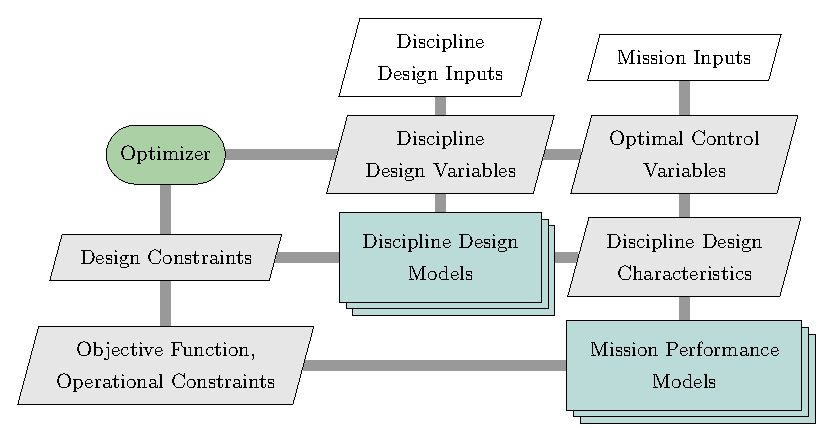
\includegraphics[scale=0.8]{../Images/General_XDSM.pdf}
 \caption{Multidisciplinary Analysis Environment.}
 \label{f:framework}
\end{center}
\end{figure}

\begin{figure}
\begin{center}
 % \textbf{!!!!! Create XDSM of Design/Static Calculations !!!!!}
 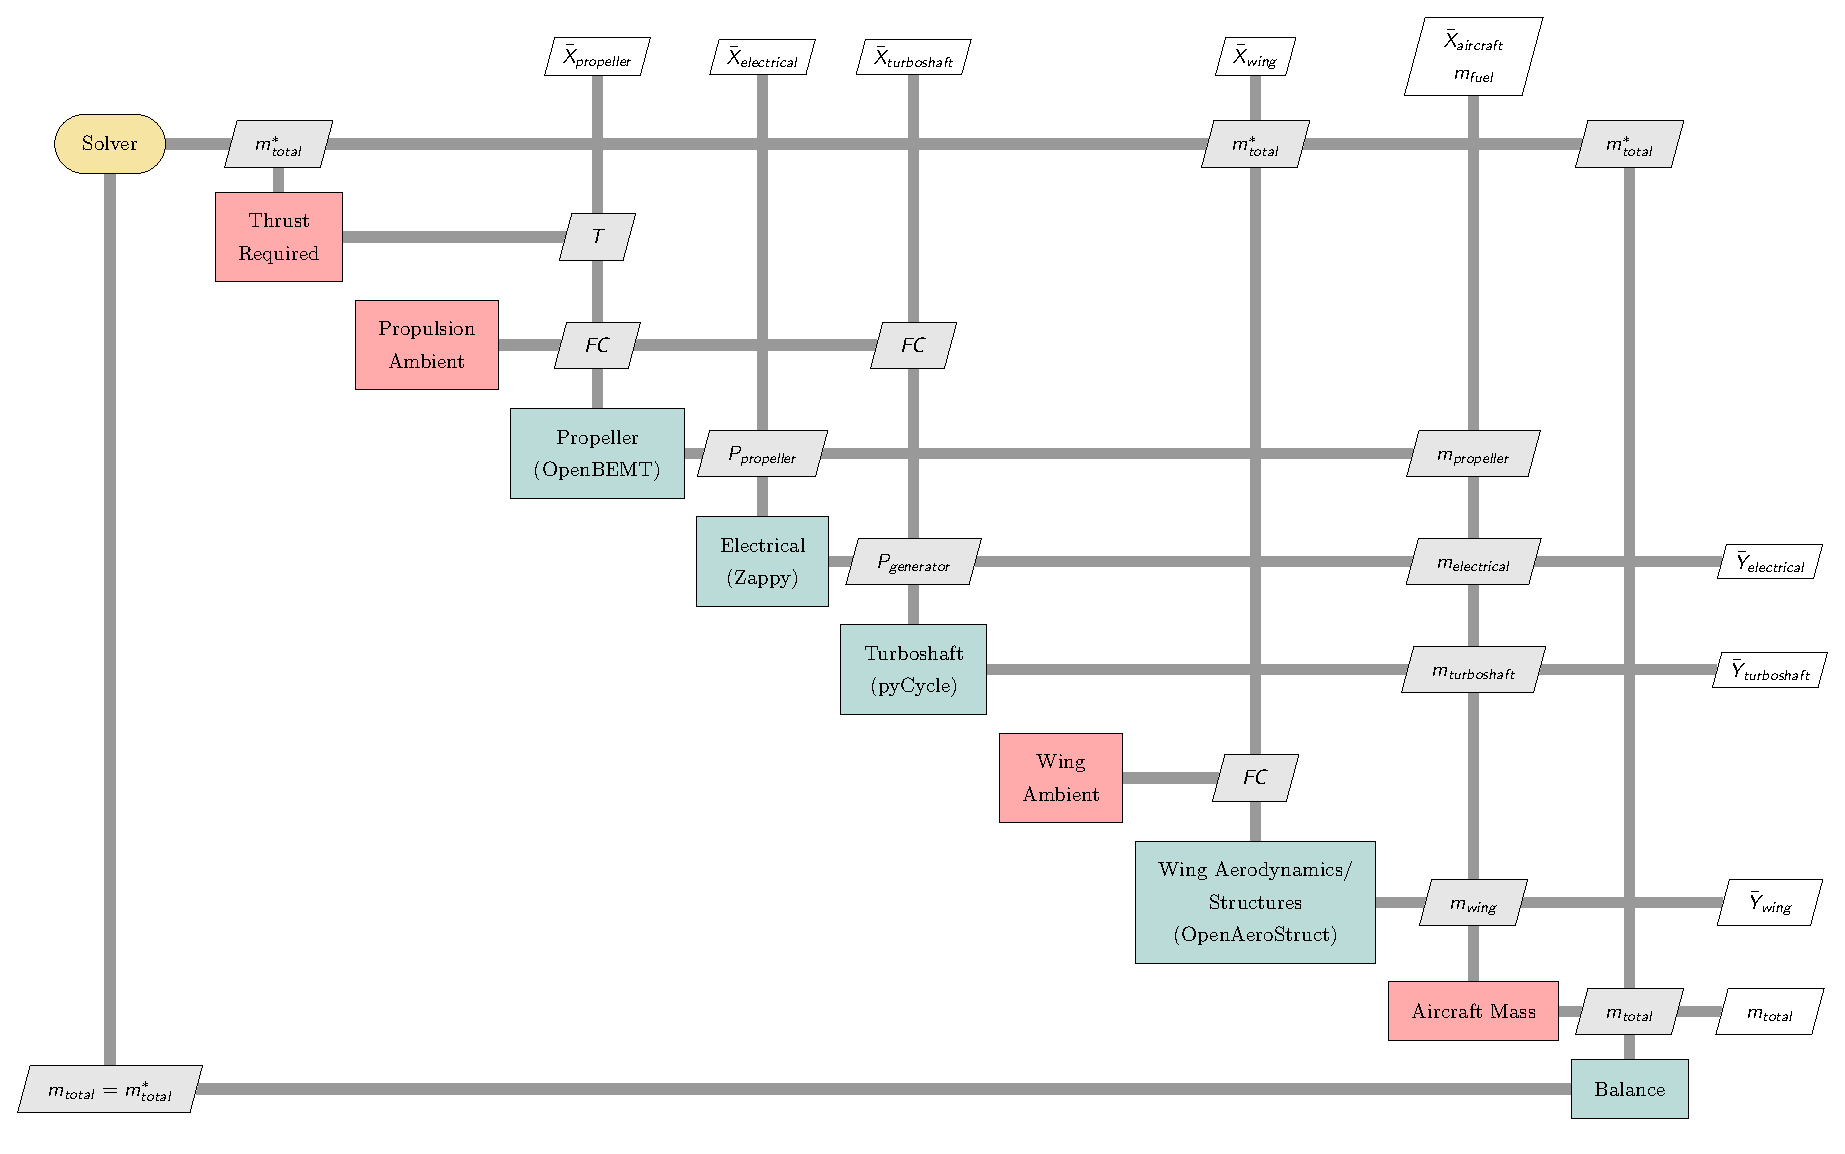
\includegraphics[width=1.0\textwidth]{../Images/Design_XDSM.pdf}
 \caption{Discipline Design Modeling.}
 \label{f:design}
\end{center}
\end{figure}

\begin{figure}
\begin{center}
 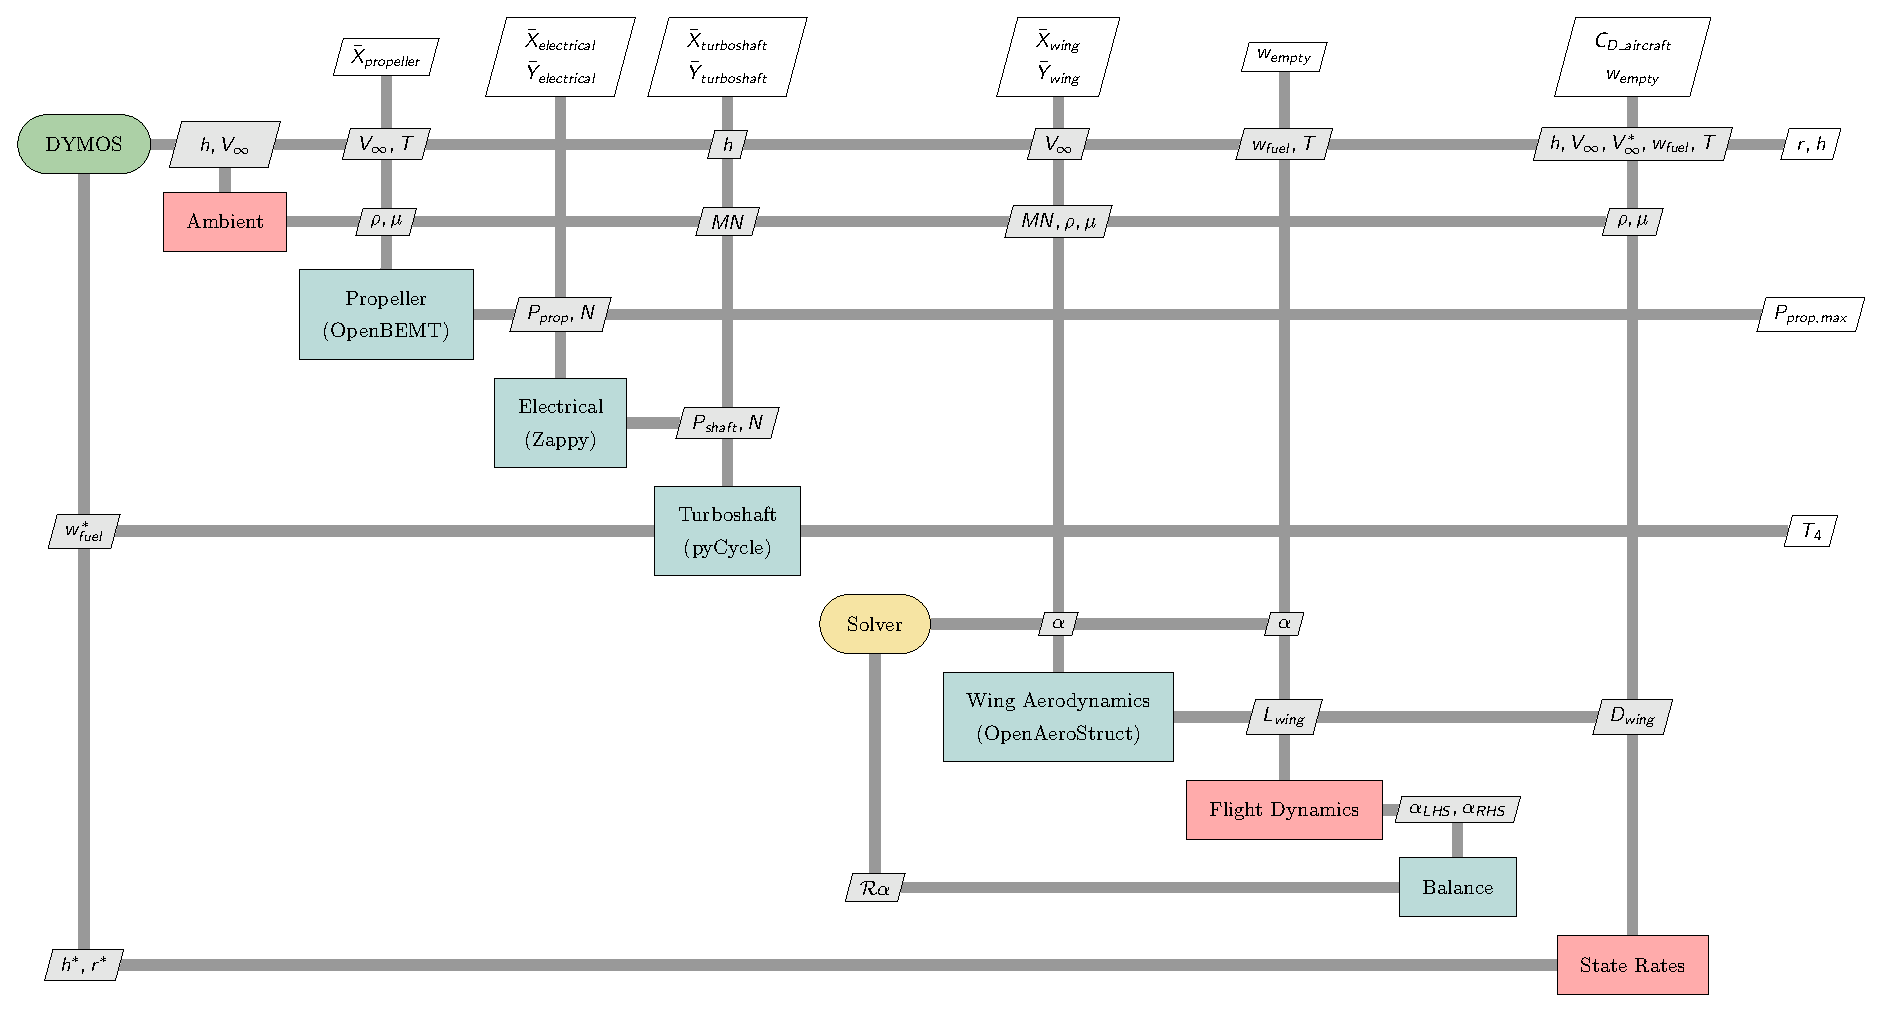
\includegraphics[width=1.0\textwidth]{../Images/Mission_XDSM.pdf}
 \caption{Mission Performance Modeling.}
 \label{f:mission}
\end{center}
\end{figure}


As can be seen in Figures \ref{f:design} and \ref{f:mission}, there are four primary disciplines included in the MDAO environment being developed in this work.  
These disciplines include propulsion, wind aerodynamics and structures, aircraft mass, and optimal control and trajectory analysis.
The next sections will describe the individual disciplinary tools created to support the above multidisciplinary design process as well as the specific models developed to represent the tiltwing vehicle under consideration in this paper.



% \begin{figure}
% \begin{center}
%  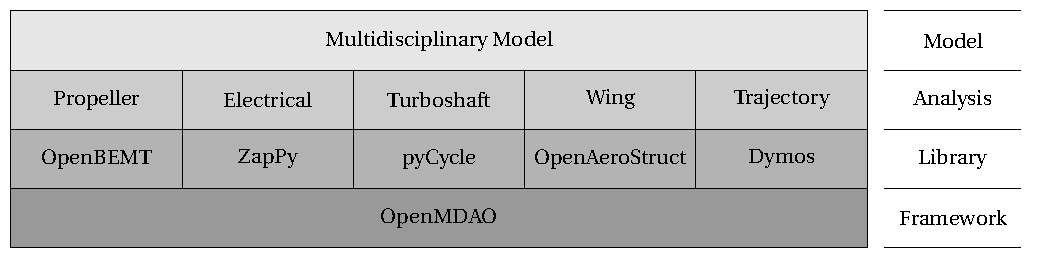
\includegraphics[width=\textwidth]{../Images/software_stack.pdf}
%  \caption{Multidisciplinary Analysis tool Softwary Stack.}
%  \label{f:stack}
% \end{center}
% \end{figure}


For each disciplinary analysis, include the foollowing information:
\begin{itemize}
    \item Describe the analysis tool and summarize the physics captured by the tool
    \item Describe the inputs and outputs of the code
    \item Make sure to include both design/static information as well as ODE information as appropriate
    \item Reference previous publications on the tool
    \item Describe the model created using the tool for the tiltwing UAM vehicle (include graphic as needed)
\end{itemize}

 %Eric, Rob, Justin, Eliot


\subsection{Propulsion System Analysis}
% this file should contain a summary of the propulsion system analysis tools and models including propeller, electric and cycle

% Summary paragraph
The propulsion systems under consideration for NASA's UAM concept vehicles cover a range of different system configurations from all-electric to turbo-electric architectures.
While the various concept vehicles consider different propulsion systems, the systems all contain similar elements leading to the developement of three supporting analysis tools and models.
These tools and models include those for the rotor or propeller, electrical system and gas turbine thermodynamic cycle, which are described in this section.  
For the tiltwing vehicle examined in this study, these three models were combined to form a propulsion system model as shown in Figure \ref{f:turboelectric}. 

% \begin{figure}
% \begin{center}
%  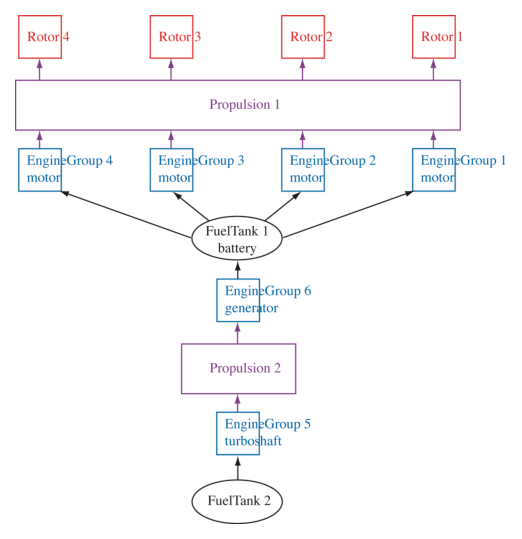
\includegraphics[width=0.6\textwidth]{../Images/Turboelectric.pdf}
%  \caption{Tiltwing Aircraft Turboelectric Propulsion System.\cite{johnson2018concept}}
%  \label{f:turboelectric}
% \end{center}
% \end{figure}


\begin{figure}
\begin{center}
 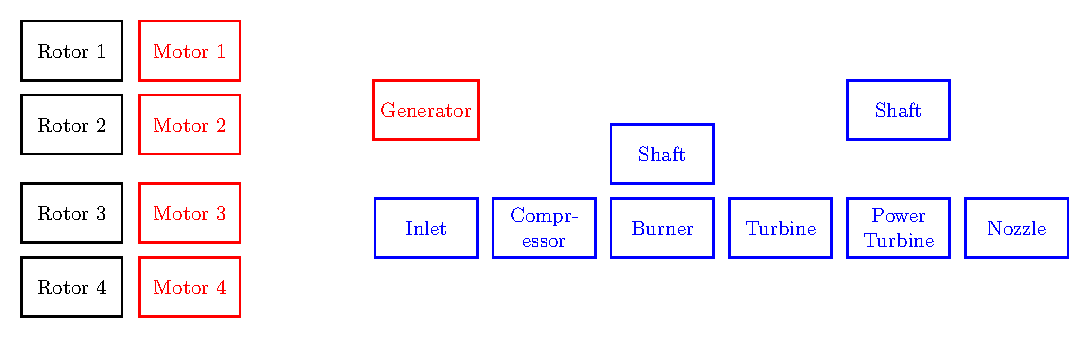
\includegraphics[width=1.0\textwidth]{../Images/Propulsion_system.pdf}
 \caption{Propulsion System Model Components.}
 \label{f:turboelectric}
\end{center}
\end{figure}

\subsubsection{Propeller Analysis} %Dan
This section needs a short summary of the propeller analysis in OpenBEMT
\begin{itemize}
    \item Describe the analysis tool and summarize the physics captured by the tool
    \item Describe the inputs and outputs of the code
    \item Make sure to include both design/static information as well as ODE information as appropriate
    \item Reference previous publications on the tool
    \item Describe the model created using the tool for the tiltwing UAM vehicle (include graphic as needed)
\end{itemize}

\subsubsection{Electrical System Analysis} %Eric



To model the electrical components of the propulsion system, a load flow analysis capability was developed on top of the OpenMDAO framework.
Load flow analysis is traditionally used by power engineers to model interconnected electrical systems such as the terrestrial AC power grid.  
However, it has also been extended to analyze DC and hybrid AC-DC systems\cite{ahmed2018generalized} as well as isolated micro-grids.
One of the benefits of the load flow method for EAP concepts is that it predicts voltages and currents throughout an electrical network given the states of distributed electric generators and loads.
This tool is actively in development and the resulting capability will be documented in a separate paper at this same conference.\cite{hendricks2019load}

\subsubsection{Thermodynamic Cycle Analysis} %Jeff, Eric
To model the gas turbine portions of the propulsion system, the recently developed thermodynamic cycle analysis tool pyCycle was selected.\cite{gray2017chemical,hearn2016optimization}
PyCycle is a new analysis tool being developed at NASA Glenn Research Center within the OpenMDAO framework.
While PyCycle is similar to other cycle analysis tools such as NPSS, its unique capability is that it provides analytic derivatives to better support gradient based solvers and optimizers.  
% This capability is enabled by developing the analysis tool within the OpenMDAO framework and taking advantage of the unified derivative methodology. 
pyCycle has been demonstrated in the context of a trajectory optimization in a previous research effort\cite{hendricks2017simultaneous} and the development of a turboshaft engine for the UAM turboelectric tiltwing aircraft will be published a this same conference.\cite{chapman2018multi}
The engine components comprising the turboshaft model for the tiltwing aircraft are shown in Figure \ref{f:turboshaft}.


 %Eric, Jeff, Dan

\subsection{Wing Aerodynamic and Structural Analysis}
% This file should contain a short summary of the aerodynamic analysis tool and models

% Summarize the physics
To model the aerostructural performance of the wing, we use OpenAeroStruct, which is an open-source tool for low-fidelity conceptual design of aircraft wings~\cite{Jasa2018a}.
OpenAeroStruct uses a vortex lattice method coupled with a six degree-of-freedom finite element method to analyze the aerostructural properties of aircraft wings.
These low-fidelity methods enable inexpensive exploration of the wing design space.
OpenAeroStruct can be used to investigate both conventional and non-conventional wings because the physics-based analyses do not rely on previously-gathered information from existing planes.
Additionally, OpenAeroStruct provides analytic derivatives for all outputs of the aerostructural analyses, which enables low cost gradient-based optimization.

% Describe the model used by this tool that was developed for the tiltwing plane
Here we use information from Johnson et al's paper, with these values specifically:
Put in table of wing design values and assumptions used
We use point masses for the engine and propellers, which was partially developed for this work

% Describe the inputs and outputs of the model and how it talks to other portions for both static and dynamic
We do both static and dynamic analysis
For static, we do a 3-point aerostructural analysis where we ensure that the wing won't fail
We choose the conditions by doing V-n analysis (cite Raymer) to determine the limiting loads of the aircraft
Include a V-n plot for a nominal flight condition

In the dynamic analysis, we only use an aerodynamic-only analysis
This is because the structural loads in the multipoint case are much more limiting
Nominally, in a regular mission, we will not come close to the structural limit of the aircraft wings
We pass the structural deformation from the 1g case to the aerodynamic cases in the dynamic analysis to get a realistically-deformed wing

\begin{figure}
\begin{center}
 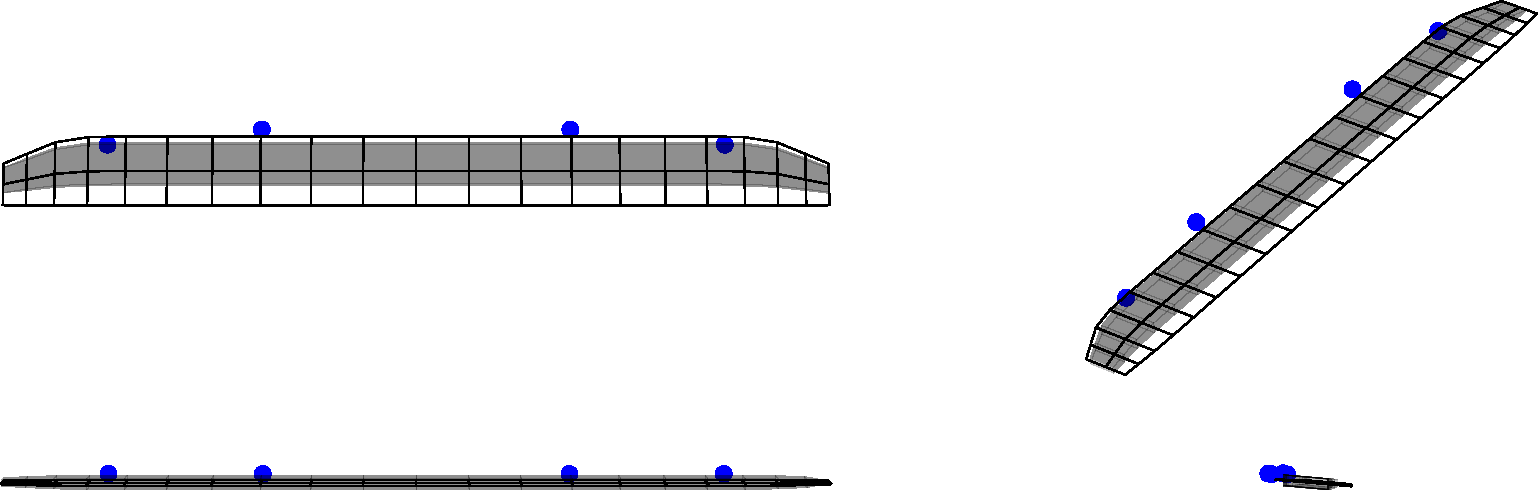
\includegraphics[width=1.0\textwidth]{../Images/aerostruct_wing}
 \caption{Isometric view of the aerostructural wing model with the engine point masses shown in blue.}
 \label{f:OAS_wing}
\end{center}
\end{figure}

\begin{figure}
\begin{center}
 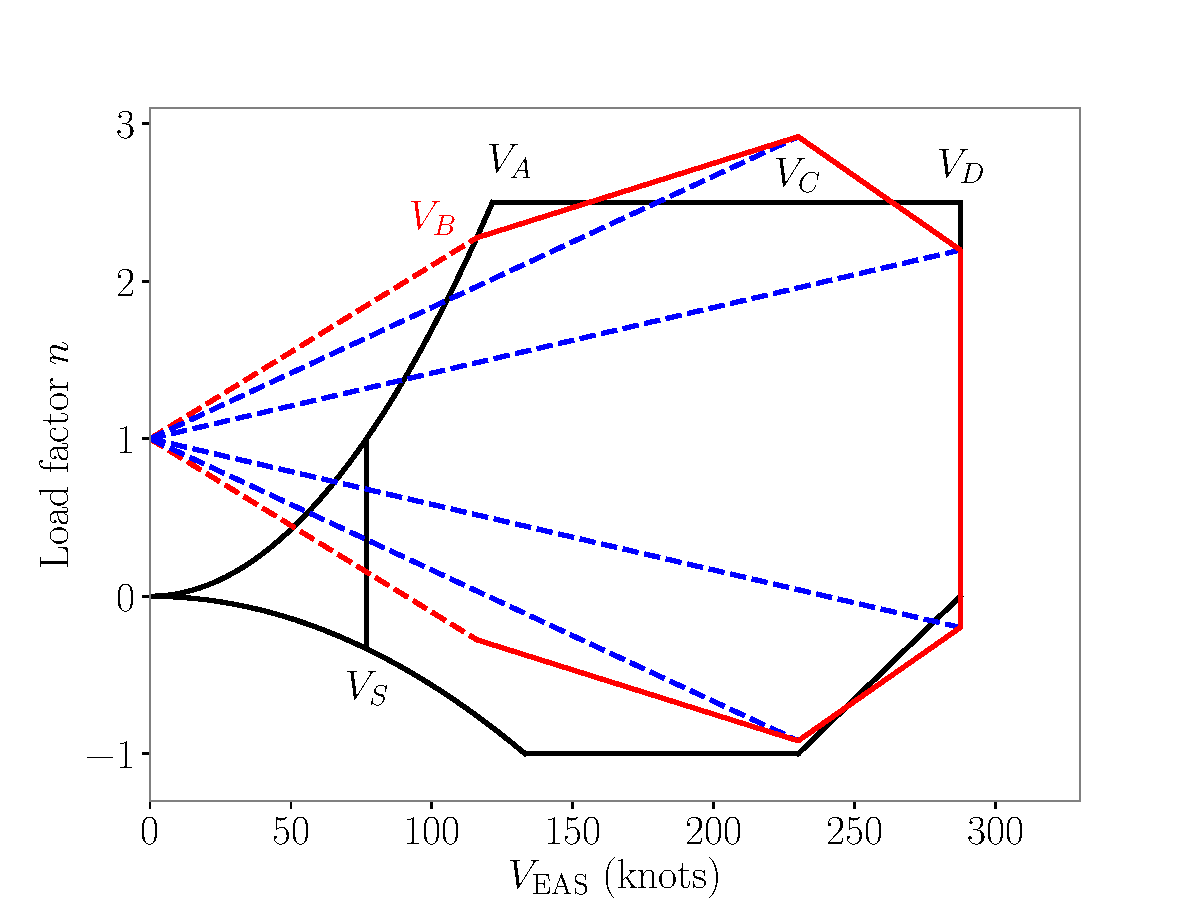
\includegraphics[width=0.7\textwidth]{../Images/v_n_diagram}
 \caption{V-n diagram used to determine the limiting flight conditions for the wing structure.}
 \label{f:v_n_diagram}
\end{center}
\end{figure}
 %John, Justin? Eliot?

\subsection{Aircraft Mass Analysis}
% This file should contain a short summary of the structures/mass analysis tool and models


Mass estimates are broken down and calculated in the following categories,
listed here by weight in descending order

\begin{itemize}

    \item engine  2055.6 lbs
    \item fuselage 1129.2 lbs
    \item wing 821.8 lbs
    \item motor 810.2 lbs
    \item drive system 715 lbs
        \begin{itemize}
            \item gearbox
        \end{itemize}
    \item fuel system 689.7 lbs
        \begin{itemize}
            \item battery
        \end{itemize}
    \item propellers 502.6 lbs
    \item landing gear 477.4 lbs
    \item cables 300 lbs
    \item tail 110.9 lbs
    \item inverter 75lbs
\end{itemize}

Engine weight was calculated based on a regression sensitive to massflow.
Drive system weight includes gearbox, rotor break, and shaft. It is derived from NDARC AFDD83 regresion based on 30 aircraft.
Fuel system weight includes tanks and supporting structures, and is based on a 15 aircraft regression.
Fuselage is based on AFDD84 NDARC universal body weight model.
Inverter weight is based on a linear regression of XX flightweight inverters.
Motor weight is based on a linear regression of XX aircraft developmental motors.
Landing gear and alighting structures are based on a regression of 28 aircraft.
Propeller weight is based on the NDARC AFDD82 model using 35 aircraft to determine hub and blade weights
Tail weight is the AFDD82 NDARC model, consistening of horizontal, vertical and tail rotor components.
Wing weight comes from OpenAeroStruct (Jasa)
Battery weight is dependent on energy capacity and energy density.
Cable weight was calculated based on a regression sensitive to current.

\cite{NDARC}

% bibtex

 %Bruce, Sydney, Jennifer? John? Justin? Eliot?

\subsection{Optimal Control and Trajectory Analysis}
% This file should contain a short summary of the trajectory analysis/optimal control tool and models

To model the trajectory of the UAM concept vehicles under consideration, the analysis tool Dymos which is written in the OpenMDAO framework was selected.\cite{falck2019optimal}
The primary capability provided by Dymos is a modular, general approach for determining optimal control schedules.
The optimal control capability applies the Legendre-Gauss-Lobatto (LGL) collocation scheme which allows for analysis with relatively few function evaluations compared to other methods.\cite{falckpointer2016}
This collocation scheme discretizes the mission into a number of segments within which a polynomial is used to specify the value of each control or  state parameter over time.
The polynomials for each state equation are defined by a set of cardinal nodes which are varied to satisfy the equations of motion at interior nodes on the function.  
By formulating the control problem in this way it can be solved with nonlinear programming approaches to determine the optimal control schedule.\cite{falckpointer2016}
Dymos has been used to evaluate the trajectory of UAM concepts coupled with acoustic analyses\cite{falck2018multi}.
 %Rob

% Include thermal section if it makes it into the optimization
% \subsection{Thermal System Analysis}
% \input{thermal} %Jeff, Sydney

% Include accoustics section if it makes it into the optimization
% \subsection{Acoustic Analysis}
% \input{acoustics} %Dan

\section{Turbo-Electric Tiltwing Optimization Demonstration Problem}\label{sec:opt_prob}
% this file should contain the formal description of the tiltwing problem that will be optimized with the described MDAO environment

This section will describe the application of the developed multidisciplinary optimization capability in the design of the turboelectric tiltwing aircraft.
A formal description of the optimization problem will be presented which will include the objective function, design variables and constraints.


% Revise this table based on the actual optimization completed
\begin{table}[!htb]
 \normalsize
 \begin{center}
  \caption{Optimization Problem Statement.}
  \label{t:opt_statement}
    \begin{tabular}{ r l l }
        \hline 
         & \textbf{Variable/Function} & \textbf{Description} \\ 
        \hline 
        minimize & $GTOW$ & Gross Takeoff Weight, lbm \vspace{1em} \\
        with respect to & $10 < OPR < 20$ & Cycle overall pressure ratio \\
         & $3000 < T_{\text{4}} < 3600$ & Combustor exit temperature, R \\
         % & $2.5 < PR_{\text{LPC,TOC}} < 4.0$ & TOC LPC pressure ratio \\
         % & $40 < OPR_{\text{TOC}} < 70$ & TOC overall pressure ratio \\
         % & $0.5 < T_{\text{ratio}} < 0.95$ & Throttle ratio ($\frac{T_{\text{4,TOC}}}{T_{\text{4,RTO}}}$) \\
         % & $1.35 < V_{\text{ratio,CRZ}} < 1.45$ & CRZ jet velocity ratio ($\frac{V_{\text{jet,core}} C_{v,\text{core}}}{V_{\text{jet,bypass}} C_{v,\text{bypass}}}$) \vspace{1em} \\
        subject to & $V_{\text{min}} > 300$ & Minimum flight speed, mph\\
         & $h_{\text{max}} < 15000$ & Maximum altitude, ft \\
        \hline
    \end{tabular}
 \end{center}
\end{table}
 %Eric, Rob, Justin, Eliot

\section{Turbo-Electric Tiltwing Optimization Demonstration Results}\label{sec:opt_results}
% This file should contain the results of our optimiztion study

The results of applying a gradient based optimization algorithm to this problem will be presented.
Insights will be drawn from these results regarding the design of UAM vehicles, specifically the tiltwing concept under consideration. 
 %Eric, Rob, Justin, Eliot

\section{Conclusion and Future Work}\label{sec:conc}
% This file should contain a conclusions from the paper and future work


This section will contain a short summary of the work presented in this paper, draw conclusions and discuss future work.

Future work:\\
-Include thermal management system models\\
-Include acoustic analysis\\
-Refine various disciplinary models\\
-Explore other conceptual designs\\
-
 %Eric, Rob, Justin


\section*{Acknowledgments}
The work presented in this paper is supported by NASA's Transformative Tools and Technologies (TTT) Project.
The authors thanks Shamsheer Chauhan for his insight into wing design and modeling.

\bibliography{References}




\end{document}
